\section{ŠUM}
Definice šumové hustoty a integrální hodnoty šumu a jejich vzájemný vztah, korelovaný a nekorelovaný příspěvek šumu, šumová charakteristika aktivních prvků (bílý a 1/f šum)

\textbf{Šum} je nežádoucí rušivý signál (napětí, proud), který má původ v tepelných a kvantových jevech. I když jde o náhodný signál, dá se poměrně dobře matematicky popsat.

\subsection{Definice šumové hustoty}
Šum lze vyjádřit i pomocí takzvané šumové spektrální hustoty. Pojem spektrální šumové
hustoty se dá dobře pochopit na principu, jakým ji měří spektrální analyzátor. Jde o pásmovou propust o velmi malé šířce pásma $\Delta$f. Tato propust „projíždí“ zvolený kmitočtový rozsah a měří při tom integrální hodnotu šumu, například napětí V\textsubscript{n}, která odpovídá „její“ šířce pásma $\Delta$f. Šumová spektrální hustota v\textsubscript{n} se pak určí vztahem:
\begin{equation}
v_{n} = \frac{V_{N}}{\sqrt{\Delta f}}
\end{equation}

\begin{figure}[h]
   \begin{center}
     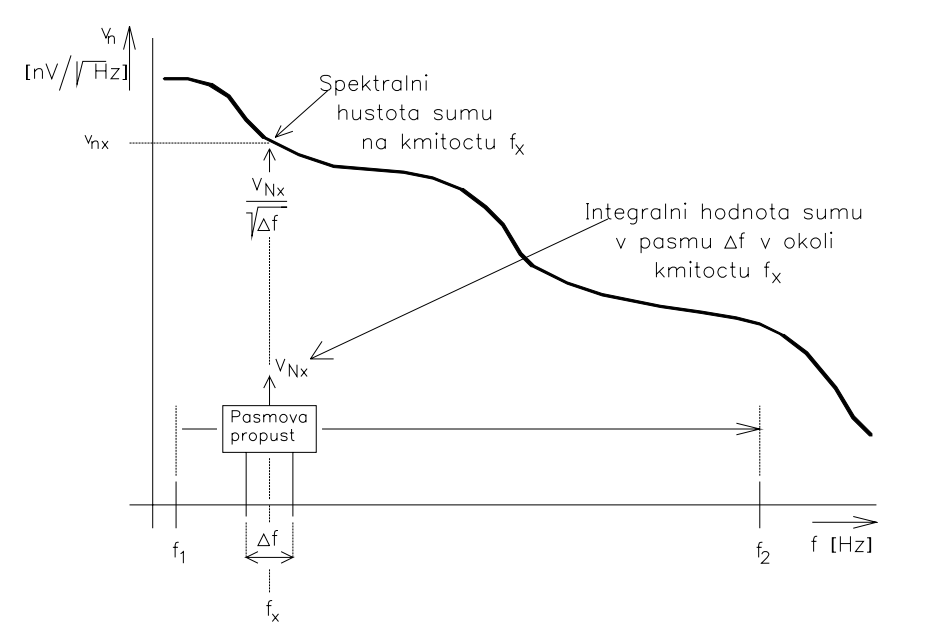
\includegraphics[scale=0.5]{images/sum.png}
   \end{center}
   \caption{Šumové spektrum}
\end{figure}

\subsection{Integrální hodnoty šumu}
Šum (například šumové napětí) se dá vyjádřit pomocí integrální hodnoty která odpovídá
definovanému kmitočtovému pásmu $\Delta$f = f\textsubscript{2} – f\textsubscript{1}. Jeho hodnota se dá prakticky změřit pomocí mikrovoltmetru, který má na vstupu pásmovou propust o lomových kmitočtech f\textsubscript{2} a f\textsubscript{1}.

\subsection{Vztah mezi spektrální šumovou hustotou a integrální hodnotou šumu
v pásmu f\textsubscript{1} – f\textsubscript{2}}
Kmitočtové pásmo f\textsubscript{1} – f\textsubscript{2} rozdělíme na diferenciály $\Delta$f podle následujícího obrázku:
\begin{figure}[h]
   \begin{center}
     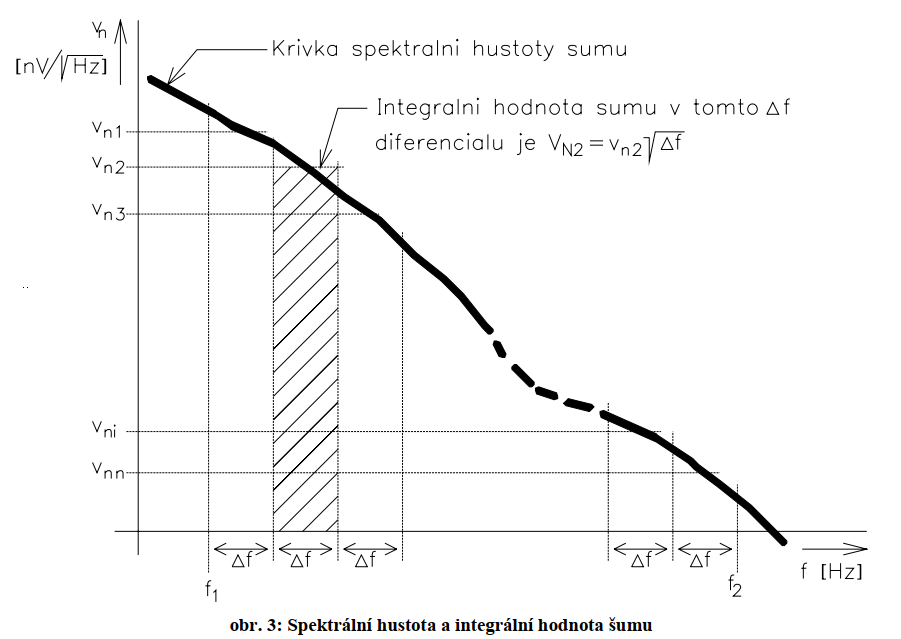
\includegraphics[scale=0.5]{images/hustota.png}
   \end{center}
   \caption{Spektrální hustota a integrální hodnota šumu}
\end{figure}

Šumové příspěvky v diferenciálech kmitočtového pásma $\Delta$f jsou na sobě nezávislé, jsou tedy nekorelované. Integrální hodnota V\textsubscript{Ni} daného diferenciálu $\Delta$f\textsubscript{i} se spočítá jako:
\begin{equation}
V_{Ni}=v_{ni}*\sqrt{\Delta f}
\end{equation}
Celková integrální hodnota šumu VN v pásmu f\textsubscript{1} – f\textsubscript{2} se pak spočítá jako součet všech nekorelovaných příspěvků odpovídajících příslušným diferenciálům $\Delta$f.

\subsection{Korelovaný a nekorelovaný příspěvek šumu}
\begin{figure}[h]
   \begin{center}
     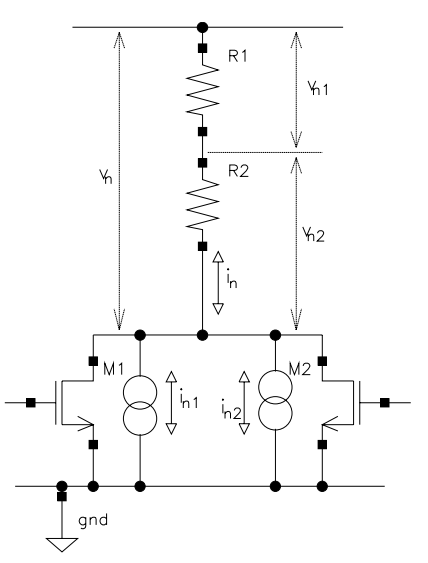
\includegraphics[scale=0.5]{images/korel.png}
   \end{center}
   \caption{Nekorelované a korelované šumové příspěvky}
\end{figure}

Šumové proudy i\textsubscript{n1} a i\textsubscript{n2} jsou na sobě nezávislé (nekorelované). Jsou to náhodné veličiny. Šumový proud i\textsubscript{n} je potom součtem \textbf{nekorelovaných} šumových proudů i\textsubscript{n1} a i\textsubscript{n2}, které se sčítají takto:
\begin{equation}
i_{n}=\sqrt{i_{n1}^2+i_{n2}^2}
\end{equation}

Pokud je hodnota šumového příspěvku menší než polovina nejvýznamnějšího příspěvku, dá se zanedbat, protože platí:

\begin{equation}
i_{n}=\sqrt{i_{n1}^2+(\frac{ i_{n2}}{2})^2} \approx 1,1 *i_{ni}\approx i_{ni}
\end{equation}

Šumový proud in protéká odpory R\textsubscript{1} a R\textsubscript{2} a na nich vytváří napěťové (šumové) úbytky v\textsubscript{n1} a v\textsubscript{n2}:
\begin{equation}
v_{n1} = R_{1}*i_{n};v_{n2}=R_{2}*i_{n}
\end{equation}
Tyto úbytky v\textsubscript{n1} a v\textsubscript{n2} jsou přímo úměrné proudu i\textsubscript{n}, jsou takzvaně \textbf{korelované} a jejich součet (šumové napětí v\textsubscript{n}) je dán prostým součtem složek v\textsubscript{n1} a v\textsubscript{n2}:
\begin{equation}
v_{n} = v_{n1}+v_{n2}=i_{n}*R_{1}+i_{n}*R_{2}=i_{n}*(R_{1}+R_{2})
\end{equation}

\subsection{Šumová charakteristika aktivních prvků (bílý a 1/f šum)}
Reálné kmitočtové spektrum šumové hustoty běžných elektronických prvků (odpory, mosové a bipolární tranzistory) má následující průběh (šumové napětí):
\begin{figure}[h]
   \begin{center}
     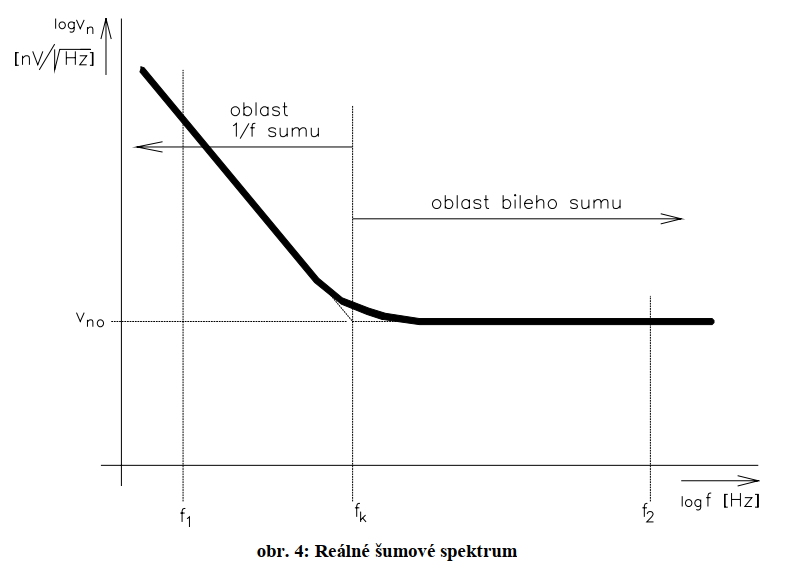
\includegraphics[scale=0.5]{images/realsum.png}
   \end{center}
   \caption{Reálné šumové spektrum}
\end{figure}

Jako oblast bílého šumu se označuje ta část kmitočtového pásma, v níž je spektrální hustota šumu konstantní, kmitočtově nezávislá (v\textsubscript{n0}). V oblasti 1/f šumu je spektrální hustota šumu nepřímo úměrná druhé odmocnině kmitočtu, tedy: 
\begin{equation}
v_{n} \approx \frac{1}{\sqrt{f}}
\end{equation}

Vztah pro šumovou hustotu v celém kmitočtovém pásmu pak má tvar:
\begin{equation}
v_{n} = v_{n0}*\sqrt{1+\frac{f_{k}}{f}}
\end{equation}
kde f\textsubscript{k} je tzv. lomová frekvence 1/f šumu

Integrální hodnota šumu V\textsubscript{N} v pásmu f\textsubscript{1} – f\textsubscript{2} je potom:
\begin{equation}
V_{N{f1-f2}}=v_{n0}*\sqrt{f_{2}+f_{k}*ln(\frac{f_{2}}{f_{1}})}
\end{equation}

Poloha lomové frekvence 1/f šumu (f\textsubscript{k}) je kritická pro nízkošumový návrh.V dané kmitočtové oblasti f\textsubscript{1} – f\textsubscript{2} by šumový příspěvek 1/f šumu měl být zanedbatelný proti šumovému příspěvku odpovídajícímu bílému šumu.

Můžeme pro zanedbání 1/f šumu odvodit:
\begin{equation}
f_{k} < \frac{0,25*f_{2}}{ln(\frac{f_{2}}{f_{1}})}
\end{equation}



